\section{Projeto de Hardware}

% // TODO: Especificações técnicas em tabelas

Com base nos requisito, foram determinados os principais componentes do projeto
para o controle e monitoramento do sistema

\subsection{Microcontrolador}

O microcontrolador Wemos D1 (figura \ref{fig:wemos}) é versátil, muito semelhante a micontroladores Arduino, e ideal para a prototipagem e foi escolhido para prototipagem do projeto. Ele possui portas de entrada e saída analógicas e digitais, fontes de alimentação de 3,3V a 5V e é programado na linguagem C. O circuito da placa foi desenvolvido tendo como base o microchip ESP8266 que oferece conectividade WiFi, diferente dos modelos mais simples de Arduino.

% \ref{fig:wemos}
\begin{figure}[h]
    \centering
    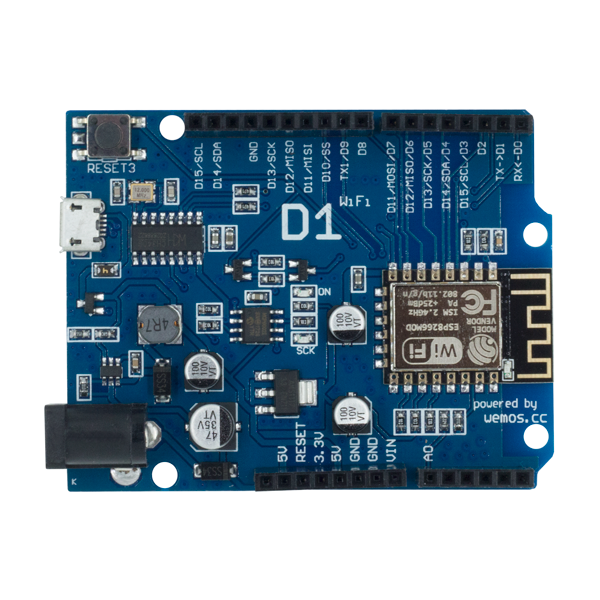
\includegraphics[scale=0.40]{figuras/projeto/hardware/wemos_d1.png}
    \captionsource{Wemos D1}{http://www.esp8266learning.com/}
    \label{fig:wemos}
\end{figure}

\subsection{Critérios de Escolha dos Sensores}

A definição dos sensores a serem utilizados se baseou nos seguintes critérios, em ordem de importância:

\begin{itemize}
    \item Faixa de operação compatível com os requisitos e especificidades do sistema
    \item Disponibilidade no mercado brasileiro
    \item Compatibilidade com o Microcontrolador
    \item Custo de aquisição
\end{itemize}

O primeiro critério é trivial, e deve ser eliminatório em qualquer avaliação. O critério de disponibilidade no mercado brasileiro teve essa classificação pelo desejo de se adquirir e trabalhar com os sensores o mais rápido possível e mitigar o risco com atrasos devido a importações e falta de estoque. A compatibilidade com o Wemos D1 exprime quão diretamente um sensor pode ser utilizado, principalmente em relação a alimentação, sendo preferíveis sensores que tenham tensões de entrada em comum com o microcontrolador, i.e., 3,3 ou 5V. Finalmente, custos de aquisição menores são preferíveis.

\subsection{Sensor de Temperatura}

Para a medição de temperatura o sensor escolhido foi o circuito integrado DS18B20 (Figura \ref{fig:ds18b20}) com uma vedação impermeável. É um sensor que atende as especificações e é amplamente utilizado em conjunto com o Wemos D1, Arduino e outros microcontroladores semelhantes, e possui alta disponibilidade no mercado a um baixo custo, sendo comercializado em uma versão impermeável, muita prática para esse projeto. A leitura da temperatura pelo microcontrolador é realizada por apenas um fio de dados, utilizando a interface One-Wire. 

Ficha técnica:
\begin{itemize}
    \item Tensão de operação: 3-5,5V
    \item Faixa de medição: -55°C a +125°C
    \item Precisão: ±0.5°C entre -10°C e +85°C
    \item Ponta de aço inoxidável
\end{itemize}

\begin{figure}[h]
    \centering
    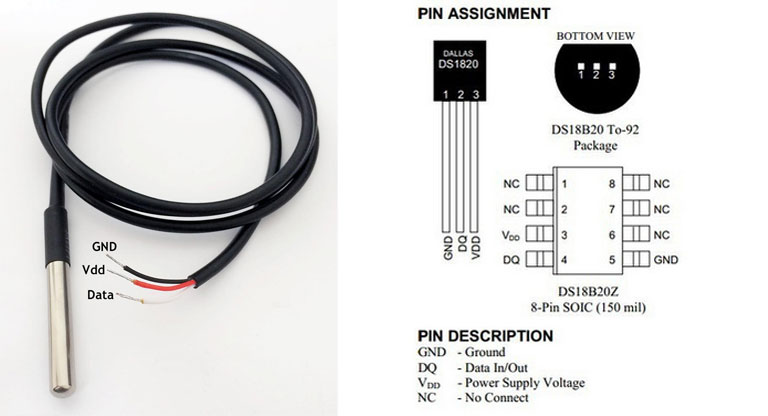
\includegraphics[scale=0.40]{figuras/projeto/hardware/ds18b20.jpg}
    \captionsource{Sensor DS18B20}{https://escapequotes.net/}
    \label{fig:ds18b20}
\end{figure}

\subsection{Sensor de Densidade Relativa}

A medição da densidade relativa é menos trivial pela ausência de sensores completos comercializados a baixo custo. Quando não é automatizada, a medição é comumente  realizada com auxílio de um densímetro ou um refratômetro, que medem a densidade relativa e a concentração de açúcar dissolvido em graus Brix, respectivamente. Ambas as ferramentas requerem interação humana e a extração de uma pequena amostra da solução, aproximadamente 100 a 250ml e algumas gotas, respectivamente.


Quanto a medição automática e contínua da densidade relativa, Boulton e Quain \cite{BoultonQuain} apresentam algumas formas de medir a grandeza, destacam-se: a utilização de sensores de pressão posicionados em diferentes alturas do fermentador, e computando a diferença de pressões medidas; e utilizando um sensor ultrassônico,  medindo o tempo que um pulso leva para ser transmitido entre dois pontos fixos, entremeado pela solução. 


Em pesquisa por soluções existentes no mercado, a abordagem de dois produtos são dignas de consideração: o Beer Bug utiliza uma célula de carga para medir o empuxo sofrido por um peso submerso na solução, e o Plaato, que utiliza a medição do gás carbônico expelido durante a fermentação para calcular indiretamente a densidade relativa.


Dentre as opções listadas, a medição por diferença de pressões e empuxo foram selecionadas para serem adotadas em primeiro momento no projeto, com prioridade da primeira. Essas são as soluções que aparentam apresentar menor complexidade na medição e maior facilidade na calibração para obtenção de resultados consistentes.


As opções listadas são discutidas a seguir, contemplando as especificações necessárias para cada sensor, e os modelos escolhidos para utilização no projeto.

\subsubsection{Medição por diferença de pressão} 

Esse método se baseia no conceito de pressão estática \(P_{estatica}\), que é pode ser calculda para um determinado ponto em um fluido como o produto da densidade \(\rho\) desse fluido, da aceleração gravitacional \(g\), e da altura \(h\) da coluna de líquido sobre o ponto escolhido.

\begin{equation}
P_{estatica} = \rho \cdot g \cdot h
\end{equation}

Consequentemente, considerando a densidade homogênea e a variação da aceleração gravitacional desprezível, a diferença de pressão entre dois pontos em diferentes alturas desse fluido, é:

\begin{equation}
\Delta P = \rho \cdot g \cdot \Delta h
\end{equation}

Dessa forma, mantendo a diferença de alturas \(\Delta h\) fixa e conhecida, é simples inferir o valor da densidade a partir da medida da diferença de pressão medida pelo sensor.


Seguindo a especificação do requisito HW-F-3, o sistema deve ser capaz de medir densidades relativas de 1,000 e 1,150, em relação à água a 20 °C, o que corresponde a uma faixa entre 998,203 e 1147,933 kg/m³. Considerando a aceleração gravitacional 9.807 m/s² e uma distância de 20 cm entre os dois pontos medidos (o que é razoável para fermentadores pequenos, até 50L), a faixa de operação do sensor de diferencial de pressão deve ser, em diferentes unidades comerciais:

\begin{table}[H]
    \begin{center}
        \begin{tabular}{ |c|c|c|c| } 
            \hline
            & N/m² ou Pa & bar & psi \\
            \hline
            Valor Mínimo & 1957,805 & 0,019578 & 0,284 \\ 
            \hline
            Valor Máximo & 2251,476 & 0,022515 & 0,327 \\ 
            \hline
        \end{tabular}
        \caption{\label{tab:densidades}Diferenças de pressão esperadas para cálculo da densidade relativa durante a fermentação.}
    \end{center}
\end{table}

Para obter a precisão de 1 milésimo de densidade relativa, o sensor necessita de uma precisão de aproximadamente 0,1\%.


A partir das especificações, foram buscados os sensores disponíveis no mercado, principalmente os produzidos pela Mouser Electronics (https://br.mouser.com/). Seguindo os critérios definidos, o modelo escolhido foi o MP3V5010DP, que é oferecido no chio Pmod DPG1 pela Diligent (Figura \ref{fig:Pmod_DPG1}), que possui as seguintes especificações:

\begin{itemize}
\item Faixa de medição: 0 a 10 kPa
\item Precisão: 5\%
\item Tensão de alimentação: 3.3V
\end{itemize}

Apesar do sensor não apresentar uma precisão adequada, acreditamos que o uso da média de diversas medidas e calibração com algumas medidas feitas pelo usuário podem propiciar resultados satisfatórios.

\begin{figure}[h]
    \centering
    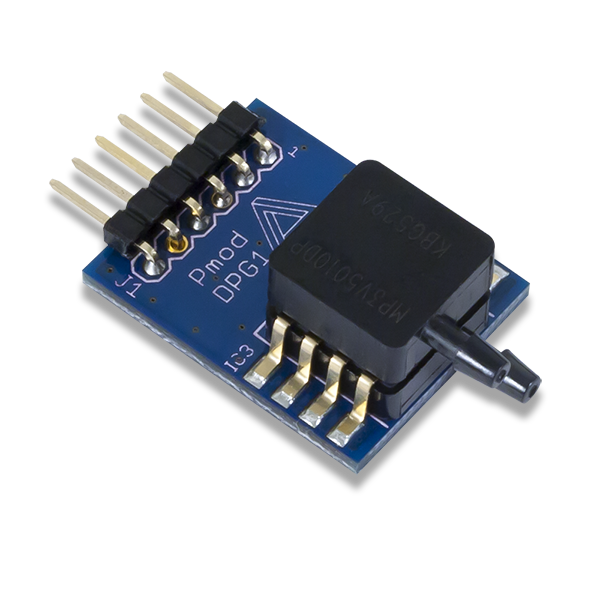
\includegraphics[scale=0.25]{figuras/projeto/hardware/DPG1.png}
    \captionsource{Sensor de diferença de pressão MP3V5010DP acoplado ao chip Pmod DPG1}{https://store.digilentinc.com/}
    \label{fig:Pmod_DPG1}
\end{figure}


\subsubsection{Medição por Empuxo}

O empuxo hidrostático \(E\) sofrido por um corpo submerso em um fluido é expresso pelo produto entre da densidade \(\rho_f\) do fluido, o volume submerso \(V_f\) do corpo, e da aceleração da gravidade \(g\): 

\begin{equation}
    E = \rho_f \cdot V_f \cdot g
\end{equation}

Naturalmente, o corpo também sofre ação da força gravitacional \(P\), que é definida pelo produto da massa \(m\) do corpo pela aceleração gravitacional \(g\):

\begin{equation}
    P = mg
\end{equation}

As duas forças atuam em sentidos opostos (como ilustrado na figura a seguir), de forma que, utilizando uma célula de carga conectada por meio de um fio a um corpo, é possível notar uma diferença no “peso natural” do objeto submerso, que é igual a força resultante entre a força gravitacional e o empuxo. Esse é o conceito de uma balança hidrostática.

\begin{figure}[h]
    \centering
    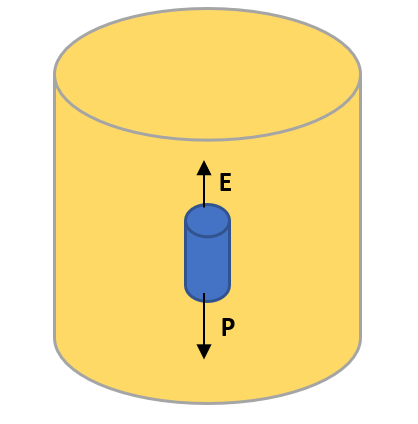
\includegraphics[scale=0.35]{figuras/projeto/hardware/empuxo.PNG}
    \captionsource{Representação de um corpo (azul) submerso em um fluido (amarelo) e das forças gravitacional e de empuxo}{Autores}
    \label{fig:empuxo}
\end{figure}

Considerando um corpo de massa 250g e volume de 125cm³ arbitrários, e a variação de densidade especificada, uma célula de carga adequada para o projeto deve ser capaz de medir massas entre 112,75 e 125,22g, com precisão mínima de aproximadamente 0,125g. Nota-se que é desejável um corpo mais denso que o fluido para que ele fique completamente submerso, facilitando aplicação da relação do empuxo. O sensor ZHIPU-200g (Figura \ref{fig:ZHIPU-200g}) foi escolhido, medindo entre 0 a 200g, com precisão de 0,1g.


\begin{figure}[h]
    \centering
    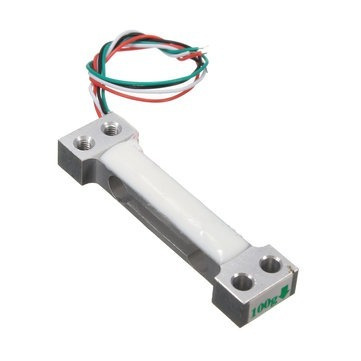
\includegraphics[scale=0.40]{figuras/projeto/hardware/ZHIPU-200g.jpg}
    \captionsource{Sensor de carga ZHIPU-200g}{https://mercadolivre.com.br/}
    \label{fig:ZHIPU-200g}
\end{figure}


\subsection{Sensor de pH}

Para a medição de pH o sensor escolhido foi o E-201-C (Figura \ref{fig:E-201-C}) com uma placa condicionadora que permite interface direta com o microcontrolador. Assim como o DS18B20, é um sensor amplamente utilizado em conjunto com o Arduino e facilmente encontrado no mercado nacional. A comunicação com o microcontrolador é realizada por comunicação serial, utilizando os protocolos UART ou I2C.


Ficha técnica:
\begin{itemize}
    \item Tensão de operação: 5V;
    \item Temperatura de operação: 0°C a 60°C;
    \item Tempo de resposta: 5s;
    \item Tempo de sedimentação: 60s;
    \item Faixa de medição: pH de 0 a 14
\end{itemize}

\begin{figure}[h]
    \centering
    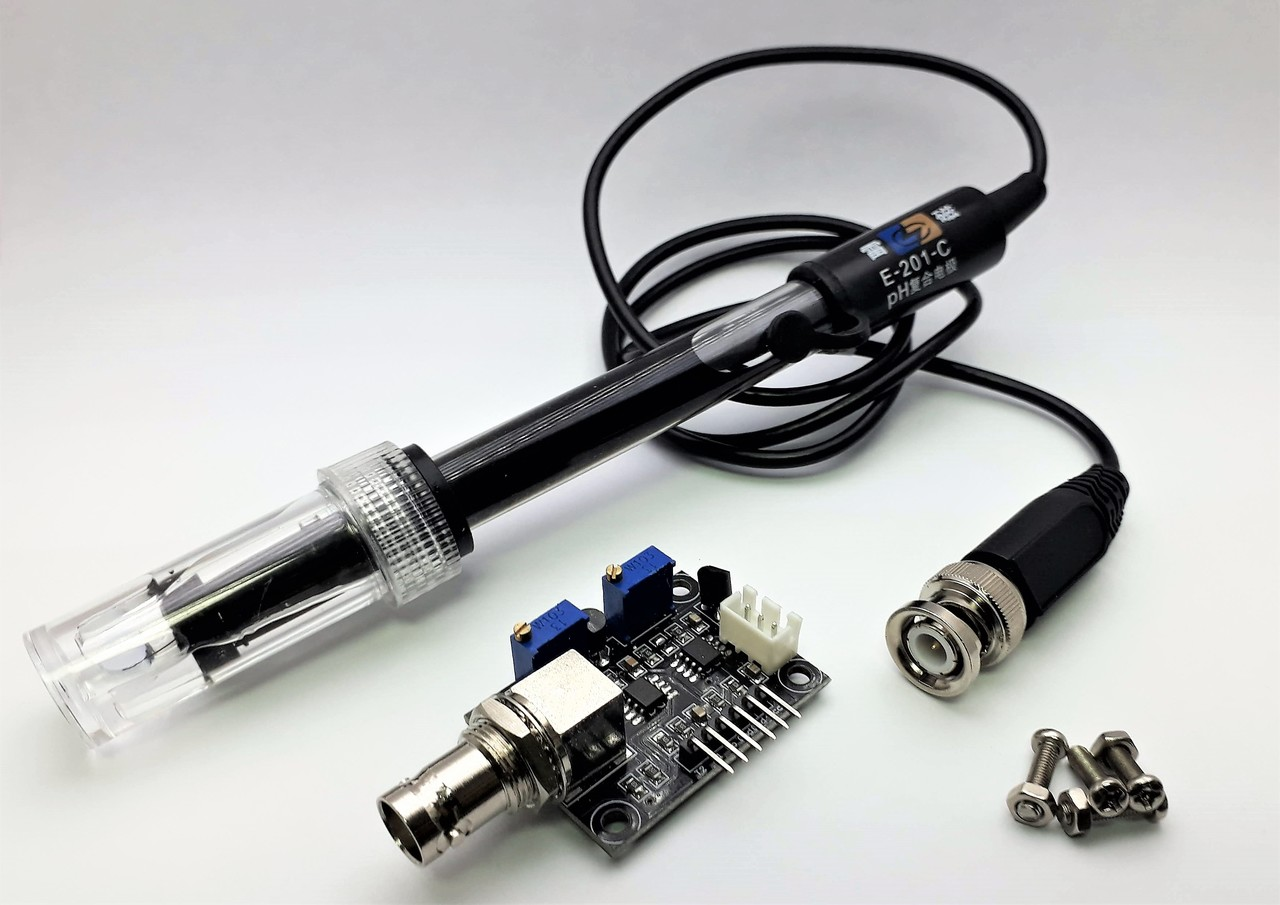
\includegraphics[scale=0.15]{figuras/projeto/hardware/E-201-C.jpg}
    \captionsource{Sensor de pH E-201-C}{https://www.crcibernetica.com/}
    \label{fig:E-201-C}
\end{figure}


\subsection{Atuador de Temperatura}

Para a montagem do nosso dispositivo que realiza trocas de calor com o fermentador, as células termoelétricas de Peltier (figura \ref{fig:peltier}) se mostraram uma boa opção. Elas são versáteis, possuem a capacidade de esfriar ou aquecer o fermentador dependendo do sentido da corrente aplicada em seus terminais e fornecem calor proporcionalmente a corrente fornecida ao sistema.


A célula é constituída por duas chapas de material isolante com um material condutor entre elas, como é esquematizado na figura \ref{fig:esquema_peltier}. Quando uma diferença de tensão é aplicada entre os terminais da célula, o movimento dos semicondutores de tipo “n” e “p” transforma a energia elétrica em energia térmica, criando um fluxo de calor que aquece uma célula e esfria outra. Em um semicondutor do tipo-n, o calor é absorvido próximo ao terminal negativo e rejeitado próximo ao terminal positivo, já em um semicondutor do tipo-p o processo se dá de maneira inversa. Como os pares tipo “n” e “p” tem características diferentes, é possível alterar o fluxo de calor dependendo do sentido da corrente.


\begin{figure}[H]
    \centering
    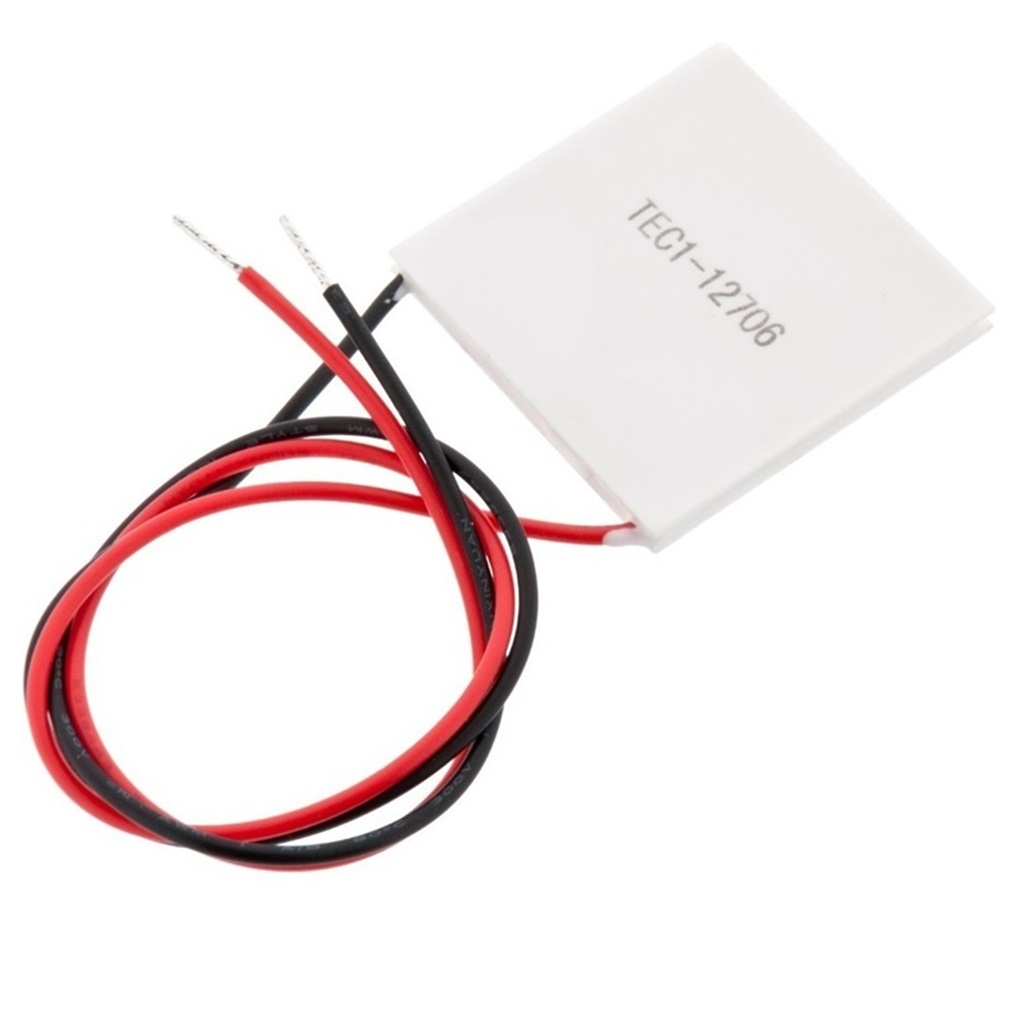
\includegraphics[scale=0.20]{figuras/projeto/hardware/pastilha_peltier.jpeg}
    \captionsource{Célula de Peltier modelo TEC1-12706.}{https://mercadolivre.com.br/}
    \label{fig:peltier}
\end{figure}

\begin{figure}[H]
    \centering
    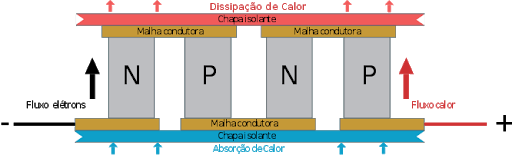
\includegraphics[scale=0.60]{figuras/projeto/hardware/peltier.png}
    \captionsource{Esquema de funcionamento de uma célula de Peltier.}{https://pt.wikipedia.org/}
    \label{fig:esquema_peltier}
\end{figure}


Um exemplo de aplicação comercial das células de Peltier para controle da temperatura de fermentação, pode ser observada no produto desenvolvido pela empresa Brew Jacket. Inspirado nessa solução, o sistema de troca de calor será composto por um dissipador de calor e uma ventoinha na face quente (figura \ref{fig:cooler}), e uma haste de aço inoxidável (figura \ref{fig:haste_inox}) ligado no lado frio, o servirá como condutor de calor entre a o fermentador e o módulo de Peltier. O aço inoxidável não conduz calor tão bem quanto o cobre ou o alumínio, mas devido resistência a corrosão em meio ácido, é a única opção segura das três.


\begin{figure}[H]
    \centering
    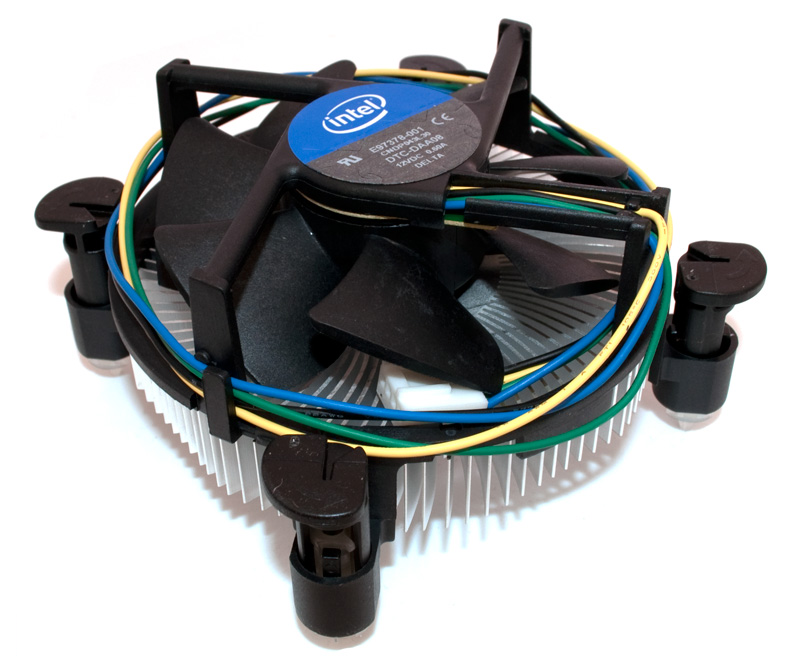
\includegraphics[scale=0.20]{figuras/projeto/controle/cooler.png}
    \captionsource{Dissipador de calor e ventoinha, modelo utilizado em CPU.}{https://www.hexus.net/}
    \label{fig:cooler}
\end{figure}


\begin{figure}[H]
    \centering
    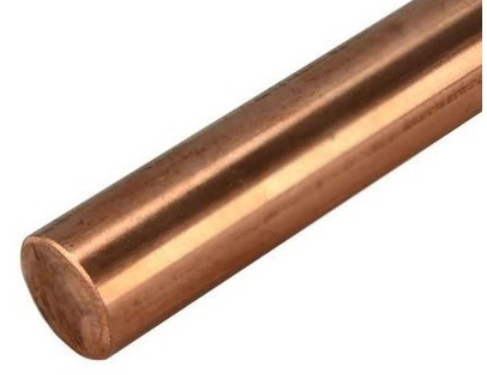
\includegraphics[scale=0.30]{figuras/projeto/controle/haste.png}
    \captionsource{Haste de Aço inoxidável.}{https://mercadolivre.com.br/}
    \label{fig:haste_inox}
\end{figure}

Uma alternativa, ainda se utilizando a célula de Peltier, é realizar a troca de calor com a solução pela parede do fermentador, de forma menos invasiva e com menores riscos de contaminação, mas gerando uma dependência maior à geometria e material do fermentador. Uma alternativa seria utilizar a células em contato próximo à parede do fermentador; e a construção de um pequeno sistema que utilize um fluido circulando por serpentinas em torno ao fermentador, com as células atuando a temperatura do fluido.

% // TODO: Diagrama do Circuito
